% !TEX root = ./BMC-Exercicios_Resolução.2.tex
\providecommand\mainfilename{"./BMC-Exercicios_Resolução.tex"}
\providecommand \subfilename{}
\renewcommand   \subfilename{"./BMC-Exercicios_Resolução.2.tex"}
\documentclass[\mainfilename]{subfiles}

\graphicspath{{\subfix{./.build/figures/BMC-Exercicios_Resolução.2/}}}
% \tikzset{external/force remake=true} % - remake all

% \date{\Large 16 de Novembro de 2022}

\begin{document}

\mymakesubfile{2}
[BMC]
{Exercicios}
{Exercicios}

\group{Lista}

\begin{questionBox}1{ % Q1
    As bases nucleotidicas absorvem radiação a \line(1,0){3em}\,\unit{\nano\metre}, enquanto que os aminoácidos aromáticos absorvem radiação a \line(1,0){3em}\,\unit{\nano\metre}.
} % Q1
    
    \begin{enumerate}[label=\alph{enumi}.]
        \begin{multicols}{4}
            \item 280, 260.
            \item 260, 280.
            \item 280, 280.
            \item 260, 260.
        \end{multicols}
        \item Nenhuma das hipóteses está correta.
    \end{enumerate}

    \paragraph*{RS:} b.

\end{questionBox}

\begin{questionBox}1{ % Q2
    Indique quais as razões de absorvância na gama dos raios ultravioleta que lhe permitem definir a pureza de uma amostra de DNA.
} % Q2

    \begin{enumerate}[label=\alph{enumi}.]
        \begin{multicols}{2}
            \item A260/A320 e A280/A260 
            \item A280/A260 e A260/A230 
            \item A230/A260eA260/A280 
            \item A260/A320 e A230/A260 
            \item A260/A280 e A260/A230
        \end{multicols}
    \end{enumerate}

    \paragraph*{RS:} e.

\end{questionBox}

\begin{questionBox}1{ % Q3
    Qual dos espectros apresentados deverá ter sido obtido a partir de uma amostra de DNA?
} % Q3
    
    \begin{center}
        \includegraphics[width=.8\textwidth]{Screenshot 2022-11-16 at 14.59.51.png}
    \end{center}

    \paragraph*{RS:} Primeiro gráfico por possuir um pico próximo de 260\,\unit{\nano\metre}

\end{questionBox}

\begin{questionBox}1{ % Q4
    O que deverá acontecer ao espectro se a amostra for fervida? Desenhe um novo espetro na figura do exercício anterior.
} % Q4

    \begin{center}
        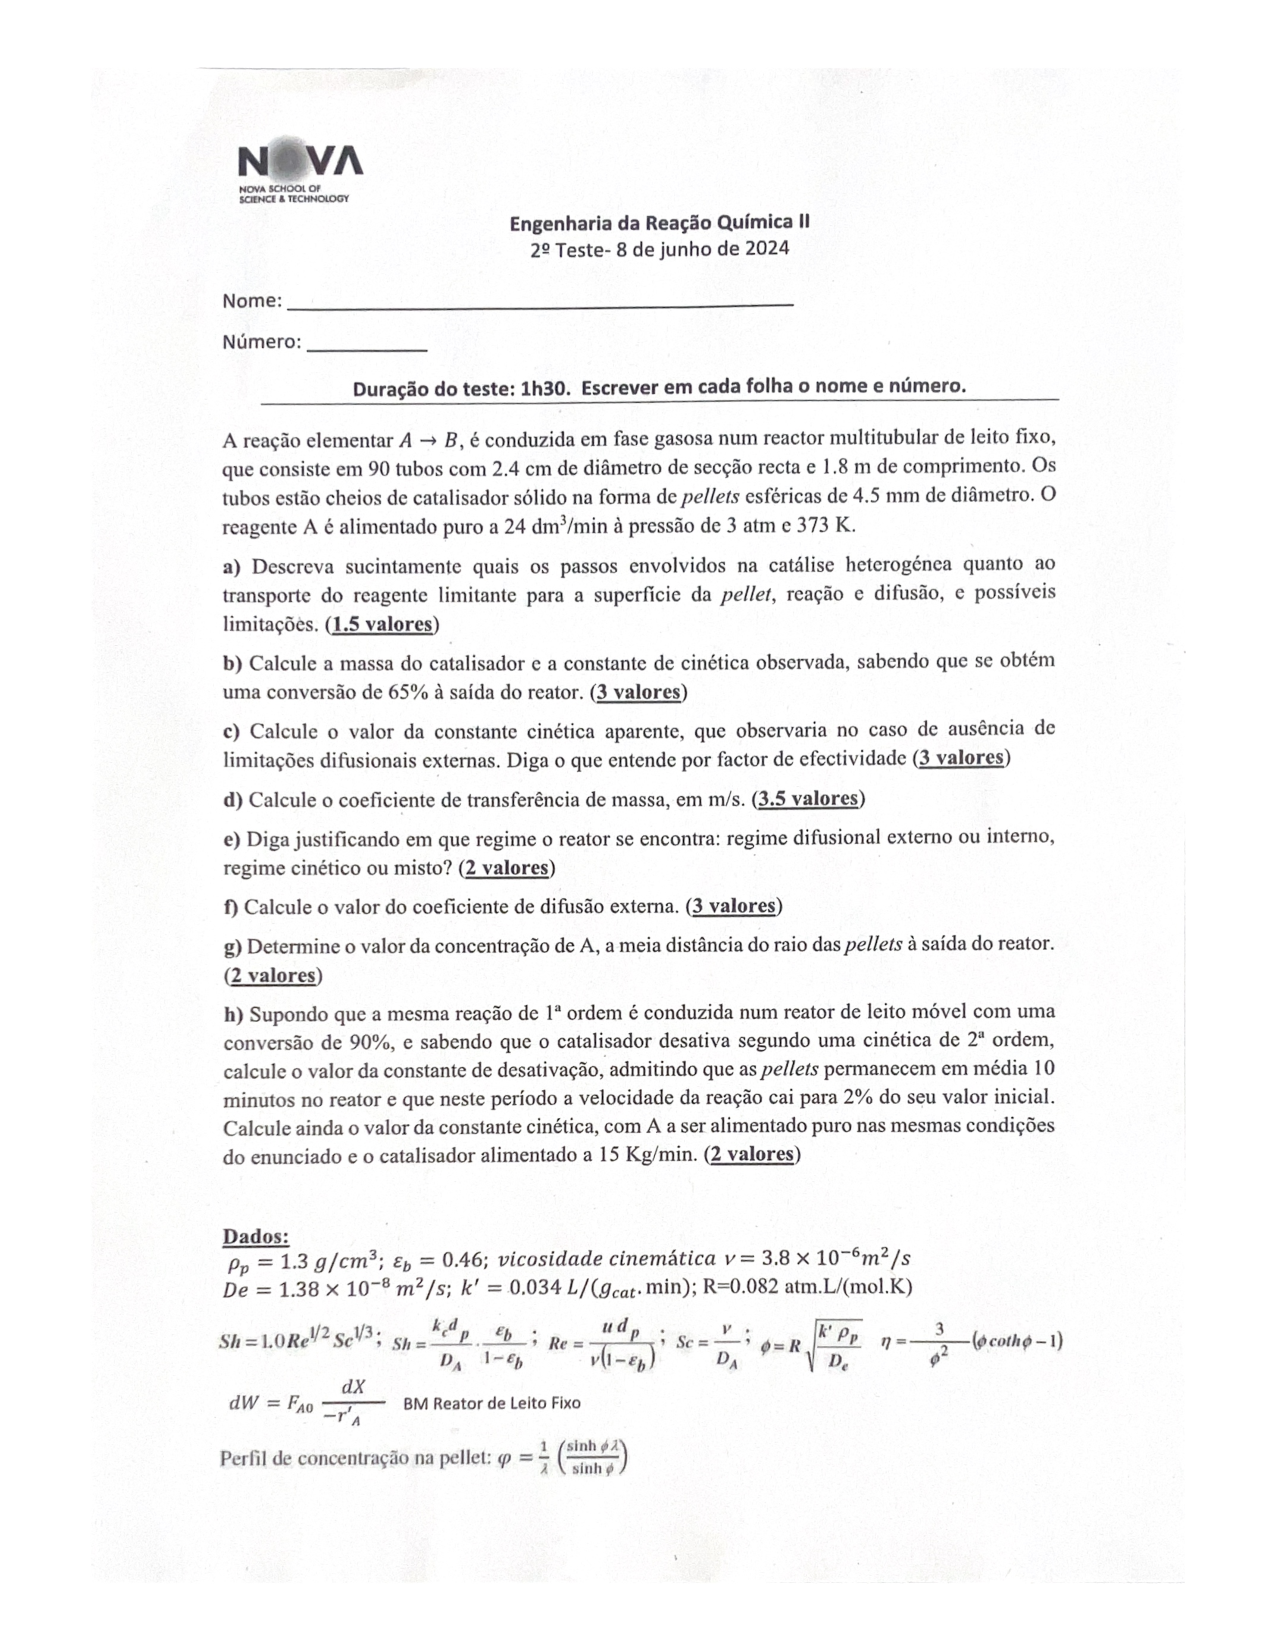
\includegraphics[width=.8\textwidth]{Scanned Document.png}
    \end{center}
    
\end{questionBox}

\begin{questionBox}1{ % Q5
    Considerando o espectro de absorvância abaixo, indique qual o valor das razões de absorvância A260/A280 e A260/A230:
} % Q5
    
    \begin{center}
        \includegraphics[width=.8\textwidth]{Screenshot 2022-11-16 at 15.00.49.png}
    \end{center}

    \paragraph*{Selecione uma opção de resposta:}
    \begin{enumerate}[label=\alph{enumi}.]
        % \begin{multicols}{1}
            \item \(A260/A280 = 0.46\) e \(A260/A230= 0.42\)
            \item \(A260/A280 = 2.15\) e \(A260/A230= 2.37\)
            \item \(A260/A280 = 0.46\) e \(A260/A230= 2.37\)
            \item \(A260/A280 = 2.15\) e \(A260/A230= 0.42\)
            \item nenhuma alínea está correta
        % \end{multicols}
    \end{enumerate}

    \begin{answerBox}{} % RS 
        \begin{flalign*}
            &
                A260/A280
                \cong 0.755/0.351
                \cong \num{2.150997150997151}
                % &\\&
                \qquad
                A260/A230
                \cong 0.755/0.318
                \cong \num{2.374213836477987}
            &
        \end{flalign*}

        \paragraph*{RS:} b.

    \end{answerBox}

\end{questionBox}

\begin{questionBox}1m{ % Q6
    Relativamente aos espetros de absorvância abaixo, indique qual a opção correta:
} % Q6
    
    \begin{center}
        \includegraphics[height=4cm]{Screenshot 2022-11-16 at 15.03.31.png}
        % \\
        \includegraphics[height=4cm]{Screenshot 2022-11-16 at 15.03.58.png}
    \end{center}
    
    \begin{enumerate}[label=\alph{enumi}.]
        \item A amostra tem muito pouco DNA.
        \item Os valores A260/A280 e A260/A230 indicam que o DNA está contaminado com proteínas com resíduos aromáticos.
        \item A amostra de DNA está contaminada com restos celulares.
        \item A amostra de DNA está contaminada com DNA em cadeia simples ou nucleotidos livres. 
        \item Os valores das razões de A260/A280 e A260/A230 estão de acordo com os critérios de pureza e o DNA plasmídico está puro.
    \end{enumerate}

    \begin{answerBox}{} % RS 
        \begin{multicols}{2}
            \paragraph*{RS 1o Gráfico:} d.\\(fazer as razões)
            \paragraph*{RS 2o Gráfico:} a.
        \end{multicols}
    \end{answerBox}

\end{questionBox}

\begin{questionBox}1{ % Q7
    No caso do espectro de absorvância obtido por espectrofotometria de UV de uma amostra de DNA plasmídico, indique qual a concentração de DNA plasmídico da amostra inicial, considerando que a leitura diz respeito a uma diluição de 1:20 da amostra inicial e que o coeficiente de extinção molar de DNA em cadeia dupla é de 20\,\unit{\milli\gram\,\milli\litre^{-1}\,\centi\metre^{-1}} e \(d=1\,\unit{\centi\metre}\).
} % Q7
    
    \begin{center}
        \includegraphics[width=.8\textwidth]{Screenshot 2022-11-16 at 15.06.32.png}
    \end{center}

    \begin{enumerate}[label=\alph{enumi}.]
        \begin{multicols}{3}
            \item 2360 \,\unit{\nano\gram/\micro\litre}
            \item 11.4 \,\unit{\nano\gram/\micro\litre}
            \item 5900 \,\unit{\nano\gram/\micro\litre}
            \item 59   \,\unit{\nano\gram/\micro\litre}
            \item 23.6 \,\unit{\nano\gram/\micro\litre}
        \end{multicols}
    \end{enumerate}

    \begin{answerBox}{C.} % RS 
        \begin{flalign*}
            &
                C 
                = C_i\,20
                = \frac{A}{L\,\varepsilon}\,20
                \cong \frac{5.9}{1*10^{-2}*20*10^{-3}}\,20
                = \frac{5.9}{20}\,20*10^{-5}
                = 5.9*10^{-5}
            &
        \end{flalign*}
    \end{answerBox}

\end{questionBox}

\begin{questionBox}1{ % Q8
    Relativamente ao espectro de absorvância obtido por espectrofotometria de UV de uma amostra de DNA plasmídico, indique qual o volume necessário de solução de DNA plasmídico inicial de forma a digerir ~2 mg de DNA, considerando que a leitura diz respeito a uma diluição de 1:100 e que o coeficiente de extinção molar de DNA em cadeia dupla é de 20\,\unit{\milli\gram\,\milli\litre^{-1}\,\centi\metre^{-1}} e \(d=1\,\unit{\centi\metre}\).
} % Q8
    
    \begin{center}
        \includegraphics[width=.8\textwidth]{Screenshot 2022-11-16 at 15.43.04.png}
    \end{center}

    \begin{enumerate}[label=\alph{enumi}.]
        \begin{multicols}{3}
            \item 0.68 \,\unit{\micro\litre}
            \item 6.8  \,\unit{\micro\litre}
            \item 68   \,\unit{\micro\litre}
            \item 59   \,\unit{\micro\litre}
            \item 5.9  \,\unit{\micro\litre}
        \end{multicols}
    \end{enumerate}

    \begin{answerBox}{C.} % RS 
        \begin{flalign*}
            &
                Vol
                = m/C
                = m\left(
                    \frac{A}{L\,\varepsilon}*100
                \right)^{-1}
                = \frac{m\,L\,\varepsilon}{A*100}
                = &\\&
                = \frac{20*10^{-2}*1*10^{-3}*20*10^{-6}}{5.900*100}
                % \cong &\\&
                \cong
                \num{67.79661016949152e-9}
            &
        \end{flalign*}
    \end{answerBox}

\end{questionBox}

\begin{questionBox}1{ % Q9
    Considerando o espectro de absorvância no UV de uma amostra de DNA obtida pelo método de extração fenólica, indique qual a explicação mais plausível para os valores de absorvância obtidos e justifique a sua escolha.
} % Q9
    
    \begin{center}
        \includegraphics[width=.8\textwidth]{Screenshot 2022-11-16 at 15.43.37.png}
    \end{center}

    \begin{enumerate}[label=\alph{enumi}.]
        \item Durante o protocolo de extração, a seguir à adição de etanol absoluto e centrifugação, o pellet soltou-se e não se conseguiu recuperar.
        \item A extração foi realizada com fenol equilibrado a pH 4.
        \item A extração foi realizada com fenol equilibrado a pH 7.
        \item Após o passo de adição da solução fenólica, a mistura não foi homogeneizada de forma eficiente, não havendo extração total da proteína.
        \item Após o passo de precipitação do DNA não se procedeu à evaporação total do álcool.
    \end{enumerate}

\end{questionBox}

\begin{questionBox}1{ % Q10
    Considerando as razões de pureza de uma amostra de DNA, analise a seguinte observação experimental:
} % Q10
    
    \begin{enumerate}[
        label={Amostra \arabic{enumi}:},
        left={0em}
    ]
        \item DNA cromossómico extraído utilizando um kit comercial, a partir de uma cultura de E. coli.\\
        \(A260/280= 1.6; A260/230=1.3\)
        \item Amostra 1, submetida a um passo de purificação fenólica (para remoção de proteínas contaminantes).\\
        \(A260/280=1.99; A260/230= 1.85\)
        \item Amostra 2, à qual se adicionou uma amostra da proteína XPTO pura.\\
        \(A260/280=1.99; A260/230=1.6\)
    \end{enumerate}

    O que pode inferir acerca da proteína XPTO?

\end{questionBox}

\group{Extra}

\begin{questionBox}1{ % Q1
    Is the sample pure or contaminated?\\
    Sample concentration in \unit{\milli\gram/\milli\litre} ?
} % Q1
    
    \begin{center}
        \includegraphics[width=.8\textwidth]{IMG_8339.JPG}
    \end{center}

    \begin{answerBox}{} % RS 
        A260/A280 = 2.1 > 2.0 e A260/A230 = 2.58 > 2.2
        \therefore\ A amostra está contaminada
        \\
        \begin{flalign*}
            &
                C
                = \frac{A}{L\,\varepsilon}*100
                = \frac{2.439}{1*10^{-2}*20*10^{-6}}*100
                = \frac{2.439}{20}
                *10^{-6}
                \cong &\\&
                \cong
                \qty{0.12195e-6}{\kilo\gram/\litre}
                = \qty{0.12195e-3}{\milli\gram/\milli\litre}
            &
        \end{flalign*}
    \end{answerBox}

\end{questionBox}

\end{document}